% =============================================================================
% Module 1c: The Schwarzschild Solution
% =============================================================================
% Sources: Carroll Ch. 5 (Secs. 5.1--5.3), Congdon & Keeton Ch. 3.3
% Mathematica: ../Mathematica/01c_Schwarzschild/
% =============================================================================

\chapter{The Schwarzschild Solution}
\label{ch:schwarzschild}

\begin{quote}
\textit{In GR, the unique spherically symmetric vacuum solution is the
Schwarzschild metric; it is second only to Minkowski space in the list of
important spacetimes.}
\hfill --- Sean Carroll, \textit{Spacetime and Geometry}
\end{quote}

\noindent
Having developed the general machinery of differential geometry in
Module~1b, we now apply it to the most important exact solution in GR:
the \textbf{Schwarzschild metric}, which describes the spacetime geometry
outside any spherically symmetric, non-rotating mass.  This metric
governs the gravitational field of stars, planets, and non-rotating
black holes, and is the starting point for understanding gravitational
lensing.

\medskip
\noindent
\textbf{Companion Mathematica files:}
\begin{itemize}[nosep]
    \item \mathlink{01c_Schwarzschild/schwarzschild_metric.wl}{schwarzschild\_metric.wl}
          --- derive and verify the Schwarzschild metric: compute
          Christoffel symbols, Riemann tensor, verify $R_{\mu\nu} = 0$,
          and compute the Kretschner scalar
    \item \mathlink{01c_Schwarzschild/gravitational_redshift.nb}{gravitational\_redshift.nb}
          --- interactive plots of gravitational redshift, time dilation,
          and Flamm's paraboloid embedding diagram
\end{itemize}

% =====================================================================
\section{The Equivalence Principle}
\label{sec:equivalence_principle}

Before diving into the Schwarzschild solution, it is worth pausing to
ask a foundational question: \textit{why} should gravity be described
by the geometry of spacetime at all?  The answer lies in the
\textbf{equivalence principle}, arguably the single most important
physical insight behind general relativity.

% ---------------------------------------------------------------------
\subsection{The Weak Equivalence Principle}
\label{sec:weak_equivalence}

The oldest form of the equivalence principle dates back to Galileo:
\textit{all objects fall at the same rate, regardless of their
composition or internal structure.}  More precisely, the
\textbf{weak equivalence principle} (WEP) states that the
\textbf{inertial mass} $m_i$ (which appears in Newton's second law,
$F = m_i\, a$) is equal to the \textbf{gravitational mass} $m_g$
(which appears in Newton's law of gravitation, $F = m_g\, g$):
\begin{equation}
    m_i = m_g \,.
    \label{eq:wep}
\end{equation}
This equality has no explanation within Newtonian mechanics --- it is
simply an empirical fact.  Yet it has been tested to extraordinary
precision: the E\"otv\"os experiments and their modern successors
(Dicke, Braginsky, and the MICROSCOPE satellite mission) have verified
eq.~\eqref{eq:wep} to better than one part in $10^{13}$:
\begin{equation}
    \frac{|m_i - m_g|}{m_g} < 10^{-13} \,.
    \label{eq:wep_precision}
\end{equation}
The universality of free fall is not an accident --- Einstein elevated
it to a \textit{principle}.

% ---------------------------------------------------------------------
\subsection{Einstein's Elevator}
\label{sec:einstein_elevator}

Einstein's great insight was to take the WEP seriously as a
fundamental principle, not merely an empirical coincidence.  He
expressed this through the famous \textbf{elevator thought experiment}:

\begin{quote}
\textit{An observer in a closed, windowless elevator cannot distinguish
between the following two situations:}
\begin{enumerate}[nosep]
    \item[(a)] \textit{The elevator is at rest on the surface of the Earth,
    where the gravitational acceleration is $g$.}
    \item[(b)] \textit{The elevator is in empty space, accelerating
    upward at $g$.}
\end{enumerate}
\end{quote}

\noindent
Conversely, an observer in free fall in a gravitational field
(``falling elevator'') experiences exactly the same conditions as
an observer floating in empty space, far from any gravitating body.
Dropped objects float alongside the observer; there is no local
experiment that can detect the gravitational field.

This equivalence between gravity and acceleration is \textit{local}:
it holds in a sufficiently small region of spacetime where tidal
effects (variations of the gravitational field across the elevator)
can be neglected.

% ---------------------------------------------------------------------
\subsection{The Strong Equivalence Principle}
\label{sec:strong_equivalence}

Einstein extended the elevator argument to its fullest form as the
\textbf{strong equivalence principle} (SEP):

\begin{quote}
\textit{The results of any local experiment (gravitational or not) in
a freely falling reference frame are indistinguishable from those of
the same experiment in special relativity.}
\end{quote}

\noindent
This has a profound consequence.  If a freely falling observer
experiences special relativity locally, then gravity cannot be a
``force'' acting in Minkowski spacetime --- it must instead be encoded
in the \textit{geometry} of spacetime itself.  Different freely falling
observers at different locations each see flat (Minkowski) spacetime
locally, but the global structure connecting these local frames is
curved.  Gravity \textit{is} the curvature of spacetime.

% ---------------------------------------------------------------------
\subsection{From the Equivalence Principle to Geodesics}
\label{sec:ep_to_geodesics}

The equivalence principle connects directly to the mathematical
framework developed in Module~1b.  A freely falling object
experiences no forces in its local (freely falling) frame --- it
follows a ``straight line'' through its local Minkowski patch of
spacetime.  But a straight line in a curved manifold is precisely a
\textbf{geodesic} (Module~1b, Section~\ref{sec:geodesics}).

Therefore, the equivalence principle implies that \textit{freely
falling particles follow geodesics of the spacetime metric}.  This
is the physical content of the geodesic equation:
\begin{equation}
    \frac{d^2 x^\mu}{d\tau^2}
    + \Gamma^\mu_{\ \alpha\beta}\,
    \frac{dx^\alpha}{d\tau}\,\frac{dx^\beta}{d\tau} = 0 \,.
    \label{eq:geodesic_ep}
\end{equation}
In Newtonian language, the Christoffel symbols $\Gamma^\mu_{\ \alpha\beta}$
play the role of gravitational ``forces,'' but in GR they are
geometric quantities --- they describe how the coordinate system
(not the particle) is ``accelerating.''

\begin{remark}
The equivalence principle tells us that gravity \textit{curves}
spacetime, but it does not tell us \textit{how} the curvature is
related to the matter content.  That information requires Einstein's
field equations $G_{\mu\nu} = 8\pi G\, T_{\mu\nu}/c^4$, which were
stated in Module~1b and whose simplest vacuum solution ($T_{\mu\nu} = 0$)
we derive in this module.  The field equations will be used throughout
the remaining modules as the foundation for gravitational lensing.
\end{remark}


% =====================================================================
\section{The Most General Spherically Symmetric Metric}
\label{sec:general_spherical}

We seek the metric outside a static, spherically symmetric mass
distribution.  The most general line element consistent with these
symmetries can be written (Carroll eq.~5.5; cf.\ Congdon \& Keeton
eq.~3.64):
\begin{equation}
    ds^2 = -e^{2\alpha(r)} dt^2 + e^{2\beta(r)} dr^2 + r^2\, d\Omega^2 \,,
    \label{eq:general_spherical}
\end{equation}
where $d\Omega^2 = d\theta^2 + \sin^2\theta\, d\phi^2$ is the metric on
the unit 2-sphere, and $\alpha(r)$ and $\beta(r)$ are functions to be
determined from Einstein's equation.

\begin{remark}
The ``static'' assumption means the metric is independent of $t$ and
has no $dt\,dr$ cross terms.  ``Spherically symmetric'' means the angular
part takes the form $r^2 d\Omega^2$, with $r$ chosen so that spheres at
constant $r$ have area $4\pi r^2$.
\end{remark}


% =====================================================================
\section{Deriving the Schwarzschild Metric}
\label{sec:schwarzschild_derivation}

We solve Einstein's vacuum equation $R_{\mu\nu} = 0$ for the
metric~\eqref{eq:general_spherical}.  The strategy follows Carroll
Sec.~5.1:

\paragraph{Step 1: Christoffel symbols.}
The nonvanishing Christoffel symbols for~\eqref{eq:general_spherical} are
(Carroll eq.~5.12):
\begin{align}
    &\Gamma^t_{\ tr} = \alpha' \,,\quad
    \Gamma^r_{\ tt} = e^{2(\alpha-\beta)}\alpha' \,,\quad
    \Gamma^r_{\ rr} = \beta' \,, \nonumber \\
    &\Gamma^r_{\ \theta\theta} = -r\,e^{-2\beta} \,,\quad
    \Gamma^r_{\ \phi\phi} = -r\,e^{-2\beta}\sin^2\theta \,, \nonumber \\
    &\Gamma^\theta_{\ r\theta} = \Gamma^\phi_{\ r\phi} = \frac{1}{r} \,,\quad
    \Gamma^\theta_{\ \phi\phi} = -\sin\theta\cos\theta \,,\quad
    \Gamma^\phi_{\ \theta\phi} = \cot\theta \,,
    \label{eq:christoffel_schwarzschild}
\end{align}
where primes denote $d/dr$.

\paragraph{Step 2: Ricci tensor.}
Computing the Ricci tensor components (Carroll eq.~5.14):
\begin{align}
    R_{tt} &= e^{2(\alpha-\beta)}\left[
        \alpha'' + (\alpha')^2 - \alpha'\beta' + \frac{2}{r}\alpha'
    \right] \,, \label{eq:Rtt} \\
    R_{rr} &= -\alpha'' - (\alpha')^2 + \alpha'\beta' + \frac{2}{r}\beta'
    \,, \label{eq:Rrr} \\
    R_{\theta\theta} &= e^{-2\beta}\bigl[r(\beta' - \alpha') - 1\bigr] + 1
    \,, \label{eq:Rthth} \\
    R_{\phi\phi} &= R_{\theta\theta}\sin^2\theta \,.
    \label{eq:Rphph}
\end{align}

\paragraph{Step 3: Solve $R_{\mu\nu} = 0$.}
From $e^{-2(\alpha-\beta)}R_{tt} + R_{rr} = 0$, we get
$\frac{2}{r}(\alpha' + \beta') = 0$, hence (Carroll eq.~5.17):
\begin{equation}
    \alpha = -\beta + \text{const} \,.
    \label{eq:alpha_beta}
\end{equation}
By rescaling the time coordinate, we set the constant to zero:
$\alpha = -\beta$.

Setting $R_{\theta\theta} = 0$ (Carroll eq.~5.18):
\begin{equation}
    e^{2\alpha}(1 + 2r\alpha') = 1 \quad\Longrightarrow\quad
    \partial_r(r\, e^{2\alpha}) = 1 \,.
    \label{eq:Rthth_zero}
\end{equation}
Integrating:
\begin{equation}
    e^{2\alpha} = 1 - \frac{R_S}{r} \,,
    \label{eq:e2alpha}
\end{equation}
where $R_S$ is an integration constant.

\paragraph{Step 4: Identify $R_S$.}
In the weak-field limit ($r \to \infty$), the metric must reduce to
$g_{tt} \approx -(1 + 2\Phi/c^2)$ with $\Phi = -GM/r$.  Comparing with
$g_{tt} = -(1 - R_S/r)$, we identify the \textbf{Schwarzschild radius}
(Carroll eq.~5.23):
\begin{equation}
    \boxed{R_S = \frac{2GM}{c^2}}
    \label{eq:schwarzschild_radius}
\end{equation}

\paragraph{Result: The Schwarzschild Metric.}
\begin{equation}
    \boxed{
    ds^2 = -\left(1 - \frac{R_S}{r}\right) c^2\, dt^2
    + \left(1 - \frac{R_S}{r}\right)^{-1} dr^2
    + r^2\, d\Omega^2
    }
    \label{eq:schwarzschild_metric}
\end{equation}
This is the unique vacuum solution with spherical symmetry
(\textbf{Birkhoff's theorem}; Carroll Sec.~5.2).  We verify $R_{\mu\nu} = 0$
symbolically in
\mathlink{01c_Schwarzschild/schwarzschild_metric.wl}{schwarzschild\_metric.wl}.


% =====================================================================
\section{Birkhoff's Theorem}
\label{sec:birkhoff}

\textbf{Birkhoff's theorem} states that the Schwarzschild metric is the
\textit{unique} spherically symmetric vacuum solution to Einstein's
equation.  The remarkable consequence: even a \textit{time-dependent}
spherically symmetric source (e.g., a pulsating star) produces a
\textit{static} exterior metric (Carroll Sec.~5.2).

This is the GR analogue of Newton's shell theorem: the gravitational
field outside a spherically symmetric mass depends only on the total
enclosed mass $M$, not on how the mass is distributed.


% =====================================================================
\section{Gravitational Time Dilation}
\label{sec:gravitational_time_dilation}

A clock at radial coordinate $r$ in the Schwarzschild spacetime runs
at a rate different from a clock at infinity.  For a stationary clock
($dr = d\theta = d\phi = 0$), the proper time is related to coordinate
time by (Congdon \& Keeton eq.~3.65):
\begin{equation}
    d\tau = \sqrt{1 - \frac{R_S}{r}}\, dt \,.
    \label{eq:grav_time_dilation}
\end{equation}
Since $\sqrt{1 - R_S/r} < 1$ for $r > R_S$, clocks closer to the mass
run \textit{slower} than clocks farther away.  At $r = R_S$, the
time dilation becomes infinite --- this is the event horizon.

\begin{figure}[ht]
    \centering
    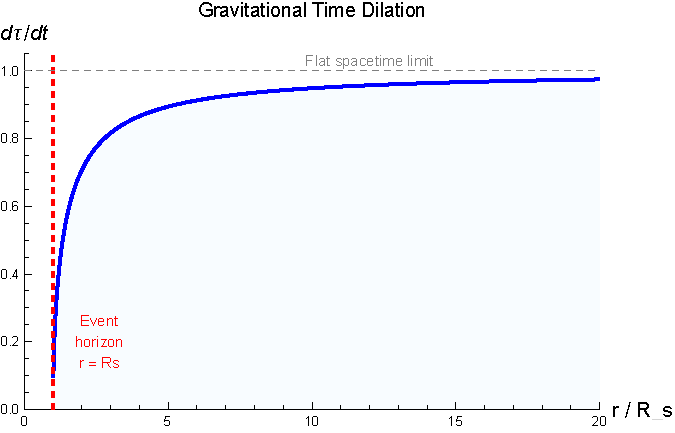
\includegraphics[width=0.65\textwidth]{../Figures/01c_Schwarzschild/time_dilation.pdf}
    \caption{Gravitational time dilation factor $d\tau/dt = \sqrt{1 - R_S/r}$
    as a function of $r/R_S$.  Clocks near the horizon ($r \to R_S$) are
    dramatically slowed.  Far from the mass ($r \gg R_S$), the factor
    approaches unity (flat spacetime).}
    \label{fig:time_dilation}
\end{figure}


% =====================================================================
\section{Gravitational Redshift}
\label{sec:gravitational_redshift}

A photon emitted at radius $r_{\mathrm{em}}$ with frequency
$\nu_{\mathrm{em}}$ is observed at $r_{\mathrm{obs}} \to \infty$ with
frequency:
\begin{equation}
    \frac{\nu_{\mathrm{obs}}}{\nu_{\mathrm{em}}}
    = \frac{\sqrt{1 - R_S/r_{\mathrm{em}}}}{\sqrt{1 - R_S/r_{\mathrm{obs}}}}
    \xrightarrow{r_{\mathrm{obs}} \to \infty}
    \sqrt{1 - \frac{R_S}{r_{\mathrm{em}}}} \,.
    \label{eq:grav_redshift}
\end{equation}
Since $\nu_{\mathrm{obs}} < \nu_{\mathrm{em}}$, the photon is
\textbf{redshifted} as it climbs out of the gravitational potential well.
The gravitational redshift parameter is:
\begin{equation}
    z_{\mathrm{grav}} = \frac{\nu_{\mathrm{em}}}{\nu_{\mathrm{obs}}} - 1
    = \left(1 - \frac{R_S}{r_{\mathrm{em}}}\right)^{-1/2} - 1 \,.
    \label{eq:grav_redshift_z}
\end{equation}
In the weak-field limit ($R_S/r \ll 1$): $z_{\mathrm{grav}} \approx GM/(rc^2)$
(Congdon \& Keeton eq.~3.63).

\begin{figure}[ht]
    \centering
    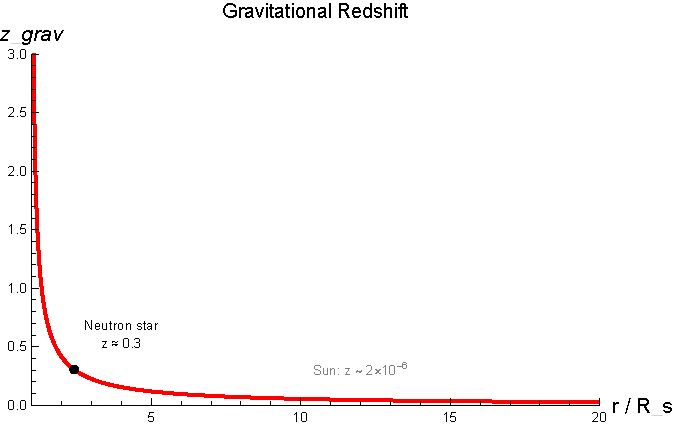
\includegraphics[width=0.65\textwidth]{../Figures/01c_Schwarzschild/gravitational_redshift.pdf}
    \caption{Gravitational redshift $z_{\mathrm{grav}}$ as a function of
    emission radius $r/R_S$.  The redshift diverges at the horizon.  The
    black dot marks a typical neutron star ($r/R_S \approx 2.4$,
    $z \approx 0.3$).  For the Sun, $z \sim 10^{-6}$.}
    \label{fig:grav_redshift}
\end{figure}

\begin{remark}
The gravitational redshift was one of the three classical tests of GR
proposed by Einstein, along with the perihelion precession of Mercury
and the bending of light.  It has been measured to high precision using
atomic clocks at different altitudes (e.g., Pound--Rebka experiment, 1959;
GPS satellite corrections).
\end{remark}


% =====================================================================
\section{The Event Horizon and Singularities}
\label{sec:event_horizon}

The Schwarzschild metric has two apparent singularities: at $r = 0$ and
at $r = R_S$.  Their nature is quite different (Carroll Sec.~5.3):

\paragraph{$r = R_S$ (coordinate singularity).}
The metric components diverge, but this is a \textit{coordinate artifact}.
The curvature remains finite, and the geometry is perfectly smooth.  In
appropriate coordinates (e.g., Eddington--Finkelstein or Kruskal--Szekeres),
the metric is regular at $r = R_S$.  However, $r = R_S$ is the
\textbf{event horizon}: once a particle crosses it, it can never return.

\paragraph{$r = 0$ (true singularity).}
This is a genuine physical singularity where the curvature becomes infinite.
We can confirm this with a curvature invariant: the
\textbf{Kretschner scalar}:
\begin{equation}
    K = R_{\mu\nu\rho\sigma}\, R^{\mu\nu\rho\sigma}
    = \frac{12\, R_S^2}{r^6}
    = \frac{48\, G^2 M^2}{c^4\, r^6} \,.
    \label{eq:kretschner}
\end{equation}
This diverges as $r \to 0$ but is finite at $r = R_S$, confirming that
only $r = 0$ is a true singularity.  We verify eq.~\eqref{eq:kretschner}
in \mathlink{01c_Schwarzschild/schwarzschild_metric.wl}{schwarzschild\_metric.wl}.


% =====================================================================
\section{Inside the Event Horizon: The Coordinate Swap}
\label{sec:dg_inside_horizon}

The Schwarzschild metric~\eqref{eq:schwarzschild_metric} describes
spacetime outside a spherical mass, but it also has something startling
to say about the region $r < R_S$.  Understanding this interior, even
briefly, sharpens our physical intuition about what the Schwarzschild
radius really means.

% ---------------------------------------------------------------------
\subsection{The Signature Flip}
\label{sec:dg_signature_flip}

Recall the Schwarzschild line element:
\[
    ds^2 = -\!\left(1 - \frac{R_S}{r}\right) c^2\, dt^2
    + \left(1 - \frac{R_S}{r}\right)^{-1} dr^2
    + r^2\, d\Omega^2 \,.
\]
Outside the horizon ($r > R_S$), the factor $f(r) \equiv 1 - R_S/r$ is
positive, so $g_{tt} < 0$ (timelike) and $g_{rr} > 0$ (spacelike).

Inside the horizon ($r < R_S$), this factor becomes \emph{negative}:
$f(r) < 0$.  Consequently:
\begin{itemize}[nosep]
    \item $g_{tt} = -f(r)\,c^2 > 0$ --- the $t$ direction is now
          \textbf{spacelike}.
    \item $g_{rr} = f(r)^{-1} < 0$ --- the $r$ direction is now
          \textbf{timelike}.
\end{itemize}
The roles of $r$ and $t$ have swapped.  Inside the horizon, $r$ is a
time coordinate and $t$ is a space coordinate.

% ---------------------------------------------------------------------
\subsection{Physical Meaning: The Singularity Is a Moment in Time}
\label{sec:dg_singularity_time}

Since $r$ is timelike inside the horizon, decreasing $r$ is the
\emph{future direction}.  Every future-directed worldline must have
$dr < 0$; the singularity at $r = 0$ is not a place you can steer
away from --- it is a \emph{moment in time} that all interior
observers inevitably reach.

\begin{remark}
You can no more avoid the singularity at $r = 0$ (once inside the
horizon) than you can avoid next Tuesday.  This is the precise sense
in which a black hole traps everything: it is not that the singularity
pulls you toward a point in space, but that the future itself points
toward $r = 0$.
\end{remark}

% ---------------------------------------------------------------------
\subsection{Why Nothing Escapes: Tilting Light Cones}
\label{sec:dg_light_cones}

For radial null rays ($ds^2 = 0$, $d\Omega = 0$) in Schwarzschild
coordinates:
\begin{equation}
    \frac{dr}{dt} = \pm\, c\left(1 - \frac{R_S}{r}\right) .
    \label{eq:radial_null}
\end{equation}
Outside the horizon, the two signs give outgoing ($+$) and ingoing ($-$)
light rays.  At $r = R_S$, both solutions give $dr/dt = 0$: light
``stands still'' in these coordinates (a coordinate effect, not a
physical one).

For $r < R_S$, the factor $(1 - R_S/r)$ is negative, so
$dr/dt$ has the \emph{same sign} for both solutions --- both
``outgoing'' and ``ingoing'' light rays have $dr < 0$ when $dt > 0$.
In other words, \textbf{all future-directed light cones point toward
smaller~$r$}.  No signal --- not even light --- can move to larger $r$
inside the horizon.

% ---------------------------------------------------------------------
\subsection{Eddington--Finkelstein Coordinates}
\label{sec:dg_eddington_finkelstein}

The pathological behavior at $r = R_S$ in Schwarzschild coordinates
is a coordinate artifact.  We can remove it by switching to
\textbf{ingoing Eddington--Finkelstein coordinates}.  Define the
advanced time coordinate:
\begin{equation}
    v = t + r_* \,, \qquad
    r_* = r + R_S \ln\!\left|\frac{r}{R_S} - 1\right| ,
    \label{eq:tortoise_and_v}
\end{equation}
where $r_*$ is the \textbf{tortoise coordinate} (Carroll eq.~5.58).
In terms of $(v, r, \theta, \phi)$, the Schwarzschild line element
becomes (Carroll eq.~5.60):
\begin{equation}
    \boxed{
    ds^2 = -\!\left(1 - \frac{R_S}{r}\right) c^2\, dv^2
    + 2c\, dv\, dr + r^2\, d\Omega^2
    }
    \label{eq:eddington_finkelstein}
\end{equation}
This metric is manifestly regular at $r = R_S$: every component is
finite and the determinant is nonzero.  The horizon is simply the
surface where outgoing light rays have $dr/dv = 0$; ingoing rays cross
it smoothly.

\begin{remark}
The Eddington--Finkelstein form makes it transparent that the event
horizon is a \emph{one-way membrane}: ingoing light ($dv > 0$,
$dr < 0$) crosses the horizon without incident, while outgoing light
at $r = R_S$ remains at $r = R_S$ forever.
\end{remark}

% ---------------------------------------------------------------------
\subsection{Relevance to Gravitational Lensing}
\label{sec:dg_interior_relevance}

\begin{remark}
For gravitational lensing, we work exclusively in the region
$r \gg R_S$ --- far outside the event horizon.  Galaxy-mass lenses
have $R_S \sim 0.1$ pc, while lensing occurs at scales of kiloparsecs.
The black hole interior is therefore not directly relevant to lensing
calculations.  Nevertheless, understanding the interior clarifies
\emph{why} the Schwarzschild radius is special (it is where light
cones tip over) and deepens physical intuition about the boundary
conditions of the exterior solution.
\end{remark}


% =====================================================================
\section{The Weak-Field Limit}
\label{sec:weak_field}

For $r \gg R_S$, the Schwarzschild metric reduces to the \textbf{weak-field}
form (Congdon \& Keeton eq.~3.71):
\begin{equation}
    ds^2 \approx -\left(1 + \frac{2\Phi}{c^2}\right) c^2 dt^2
    + \left(1 - \frac{2\Phi}{c^2}\right)
    \bigl[dr^2 + r^2\, d\Omega^2\bigr] \,,
    \label{eq:weak_field}
\end{equation}
where $\Phi = -GM/r$ is the Newtonian gravitational potential.  This
form is valid for \textit{any} weak gravitational field, not just the
Schwarzschild case, and will be the starting point for deriving the
deflection angle of light in Module~2.

\begin{remark}
The weak-field metric~\eqref{eq:weak_field} has an important feature:
the spatial part is modified by a factor $(1 - 2\Phi/c^2)$ as well as
the time part.  This means that gravity affects both the \textit{rate}
of clocks (time dilation) and the \textit{curvature of space}.
Both effects contribute equally to the bending of light --- this is why
GR gives twice the Newtonian deflection angle.
\end{remark}


% =====================================================================
\section{Isotropic Coordinates}
\label{sec:isotropic_coords}

The standard Schwarzschild coordinates $(t, r, \theta, \phi)$ have
an important asymmetry: the radial and angular parts of the spatial
metric carry \textit{different} factors.  In
eq.~\eqref{eq:schwarzschild_metric}, the $dr^2$ term is multiplied by
$(1 - R_S/r)^{-1}$ while the angular part $r^2\,d\Omega^2$ has no such
factor.  The spatial part of the Schwarzschild metric is therefore
\textit{not} conformally flat --- it is not proportional to the
flat-space metric $dr^2 + r^2\,d\Omega^2$.

We can remedy this by introducing \textbf{isotropic coordinates}, in
which the spatial metric \textit{is} conformally flat.

\subsection{The Isotropic Radial Coordinate}

Define a new radial coordinate $\rho$ via:
\begin{equation}
    r = \rho\left(1 + \frac{R_S}{4\rho}\right)^{\!2} .
    \label{eq:isotropic_r}
\end{equation}
This transformation is invertible for $r > R_S$ (i.e., outside the
event horizon), with the inverse
$\rho = \tfrac{1}{2}(r - R_S/2 + \sqrt{r^2 - r\,R_S})$.

\subsection{The Schwarzschild Metric in Isotropic Form}

In the coordinates $(t, \rho, \theta, \phi)$, the Schwarzschild
metric becomes:
\begin{equation}
    \boxed{
    ds^2 = -\left(\frac{1 - R_S/(4\rho)}{1 + R_S/(4\rho)}\right)^{\!2}
    c^2\, dt^2
    + \left(1 + \frac{R_S}{4\rho}\right)^{\!4}
    \bigl(d\rho^2 + \rho^2\, d\Omega^2\bigr)
    }
    \label{eq:schwarzschild_isotropic}
\end{equation}
The crucial feature is that the spatial part is now proportional to
the \textit{flat-space metric} $d\rho^2 + \rho^2\,d\Omega^2$ ---
the spatial geometry is \textbf{conformally flat}.  The single
conformal factor $(1 + R_S/(4\rho))^4$ multiplies all three spatial
directions equally, hence the name ``isotropic.''

\subsection{Weak-Field Expansion}

To first order in $R_S/\rho$ (the weak-field regime $\rho \gg R_S$),
the isotropic metric reduces to:
\begin{equation}
    ds^2 \approx -\left(1 - \frac{R_S}{2\rho}\right) c^2\, dt^2
    + \left(1 + \frac{R_S}{2\rho}\right)
    \bigl(d\rho^2 + \rho^2\, d\Omega^2\bigr) .
    \label{eq:isotropic_weak_field}
\end{equation}
Since $R_S = 2GM/c^2$, we have $R_S/(2\rho) = GM/(\rho\, c^2) =
-\Phi/c^2$ where $\Phi = -GM/\rho$ is the Newtonian potential.
Equation~\eqref{eq:isotropic_weak_field} is therefore:
\begin{equation}
    ds^2 \approx -\left(1 + \frac{2\Phi}{c^2}\right) c^2\, dt^2
    + \left(1 - \frac{2\Phi}{c^2}\right)
    \bigl(d\rho^2 + \rho^2\, d\Omega^2\bigr) ,
    \label{eq:isotropic_newtonian}
\end{equation}
which is precisely the weak-field metric~\eqref{eq:weak_field} with
$r$ replaced by $\rho$.  (In the weak-field regime, $r$ and $\rho$
agree to leading order.)

\subsection{Connection to the Linearized Gravity Formalism}

This result provides the explicit \textbf{bridge} between the exact
Schwarzschild solution (this module) and the linearized gravity
approach (Module~1e).  In Module~1e, the weak-field metric is derived
from first principles as a perturbation of flat spacetime:
$g_{\mu\nu} = \eta_{\mu\nu} + h_{\mu\nu}$ with
$h_{00} = -2\Phi/c^2$ and $h_{ij} = -2\Phi/c^2\,\delta_{ij}$.
The isotropic form~\eqref{eq:isotropic_newtonian} shows that the
Schwarzschild solution, when expanded to first order, reproduces
exactly this linearized metric.  The two descriptions --- exact
solution in curved coordinates, and perturbation theory in nearly
flat coordinates --- describe the \textit{same physics} in different
coordinate systems.

\begin{remark}
The isotropic form makes the connection to the parameterized
post-Newtonian (PPN) formalism and the factor-of-2 in light
deflection transparent.  In eq.~\eqref{eq:isotropic_newtonian}, both
$h_{00} = -2\Phi/c^2$ (time perturbation) and
$h_{ij} = -2\Phi/c^2\,\delta_{ij}$ (space perturbation) are
proportional to $R_S/\rho$, confirming that the time and space
perturbations are \textit{equal}.  In the PPN formalism, this
equality corresponds to $\gamma_{\mathrm{PPN}} = 1$, which is the GR
prediction.  As we saw in the weak-field limit discussion, this equal
contribution of time and space curvature is precisely why GR predicts
\textit{twice} the Newtonian deflection angle for light.
\end{remark}


% =====================================================================
\section{Schwarzschild Radius for Astrophysical Objects}
\label{sec:RS_examples}

\begin{center}
\begin{tabular}{llll}
\toprule
\textbf{Object} & \textbf{Mass} & $R_S$ & \textbf{Actual Radius} \\
\midrule
Earth   & $6 \times 10^{24}$ kg  & 8.9 mm     & 6371 km \\
Sun     & $2 \times 10^{30}$ kg  & 3.0 km     & $7 \times 10^5$ km \\
Neutron star & $1.4\,\Msun$      & 4.1 km     & $\sim 10$ km \\
SgrA*   & $4 \times 10^6\,\Msun$ & $1.2 \times 10^7$ km & --- (black hole) \\
Galaxy ($10^{12}\,\Msun$) & $10^{12}\,\Msun$ & $3 \times 10^{12}$ km & --- \\
\bottomrule
\end{tabular}
\end{center}

For a galaxy-mass lens ($M \sim 10^{12}\, \Msun$), $R_S \sim 0.1$ pc ---
far smaller than the galaxy itself.  This confirms that the weak-field
limit is appropriate for gravitational lensing by galaxies.


% =====================================================================
\section{Embedding Diagram: Flamm's Paraboloid}
\label{sec:flamm}

To visualize the spatial curvature of the Schwarzschild geometry, we can
embed the equatorial ($\theta = \pi/2$) spatial slice in 3D Euclidean space.
At constant time $t$, the spatial metric on the equatorial plane is:
\begin{equation}
    dl^2 = \left(1 - \frac{R_S}{r}\right)^{-1} dr^2 + r^2\, d\phi^2 \,.
    \label{eq:equatorial_metric}
\end{equation}
Embedding this as a surface of revolution $z(r)$ in cylindrical coordinates
$(r, \phi, z)$ where $dl^2 = (1 + z'^2) dr^2 + r^2 d\phi^2$, we find:
\begin{equation}
    z(r) = 2\sqrt{R_S}\,\sqrt{r - R_S} \,,
    \label{eq:flamm}
\end{equation}
which is \textbf{Flamm's paraboloid} (Figure~\ref{fig:flamm}).

\begin{figure}[ht]
    \centering
    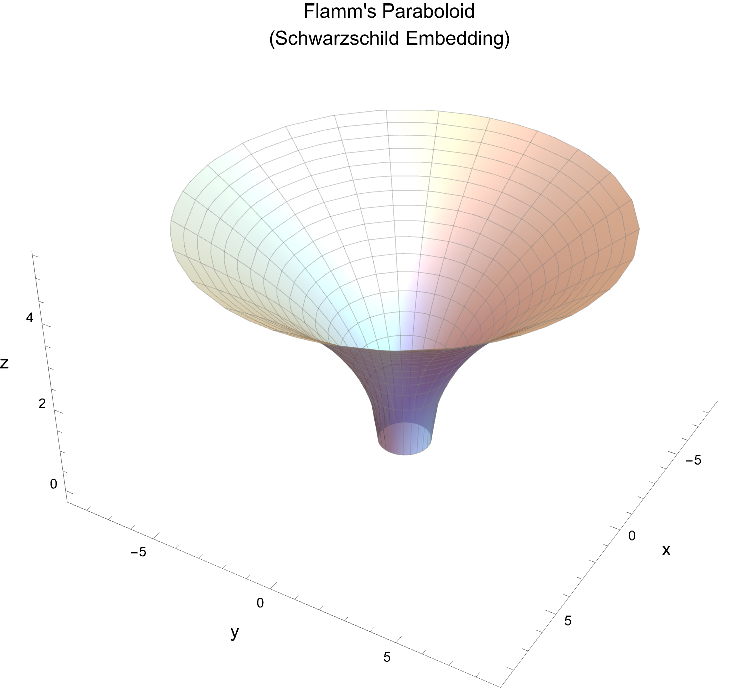
\includegraphics[width=0.7\textwidth]{../Figures/01c_Schwarzschild/flamm_paraboloid.pdf}
    \caption{Flamm's paraboloid: the equatorial spatial geometry of the
    Schwarzschild spacetime embedded in 3D Euclidean space.  The throat
    at $r = R_S$ represents the event horizon.  The surface curves more
    steeply near the throat, visualizing the spatial curvature caused by
    gravity.  An interactive version is in
    \texttt{gravitational\_redshift.nb}.}
    \label{fig:flamm}
\end{figure}


% =====================================================================
\section{Summary}
\label{sec:schwarzschild_summary}

\begin{itemize}
    \item The Schwarzschild metric is the unique spherically symmetric
          vacuum solution (Birkhoff's theorem).
    \item It is parameterized by a single quantity: the mass $M$
          (or equivalently the Schwarzschild radius $R_S = 2GM/c^2$).
    \item Gravitational time dilation: clocks run slower in stronger
          gravitational fields; $d\tau = \sqrt{1 - R_S/r}\, dt$.
    \item Gravitational redshift: photons lose energy climbing out
          of a potential well.
    \item $r = R_S$ is a coordinate singularity (event horizon);
          $r = 0$ is a true curvature singularity.
    \item The weak-field limit
          ($ds^2 \approx -(1 + 2\Phi/c^2)c^2 dt^2 + (1 - 2\Phi/c^2) d\ell^2$)
          will be the foundation for light deflection in Module~2.
\end{itemize}


% =====================================================================
\section{Problems}
\label{sec:schwarzschild_problems}

\begin{exercise}
\label{ex:verify_vacuum}
Using the reusable functions from Module~1b
(\mathlink{01b_Differential_Geometry/christoffel_symbols.wl}{christoffel\_symbols.wl}),
verify that the Schwarzschild metric~\eqref{eq:schwarzschild_metric}
satisfies $R_{\mu\nu} = 0$.
\end{exercise}

\begin{exercise}
\label{ex:kretschner}
Compute the Kretschner scalar $K = R_{\mu\nu\rho\sigma}R^{\mu\nu\rho\sigma}$
for the Schwarzschild metric and show that $K = 12\,R_S^2/r^6$.
Verify that $K$ is finite at $r = R_S$ but diverges at $r = 0$.
\end{exercise}

\begin{exercise}
\label{ex:schwarzschild_radii}
Compute the Schwarzschild radius for:
\begin{enumerate}[label=(\alph*)]
    \item The Earth ($M = 5.97 \times 10^{24}$ kg)
    \item The Sun ($M = 1.99 \times 10^{30}$ kg)
    \item A typical galaxy lens ($M = 10^{12}\, \Msun$)
\end{enumerate}
In each case, compare $R_S$ to the physical size of the object.
\end{exercise}

\begin{exercise}
\label{ex:grav_redshift_calc}
A photon is emitted from the surface of a neutron star ($M = 1.4\,\Msun$,
$R = 10$ km).
\begin{enumerate}[label=(\alph*)]
    \item Compute the gravitational redshift $z_{\mathrm{grav}}$.
    \item By what fraction is the photon's wavelength increased by the time
          it reaches a distant observer?
    \item Compare to the redshift from the surface of the Sun.
\end{enumerate}
\end{exercise}

\begin{exercise}
\label{ex:flamm_derive}
Derive the Flamm's paraboloid embedding~\eqref{eq:flamm} by embedding the
equatorial spatial slice of the Schwarzschild geometry in 3D Euclidean
space with cylindrical coordinates $(r, \phi, z)$.
\end{exercise}
